\subsection{Implementation}

Formålet med dette afsnit er at give en beskrivelse af programmets opbygning og struktur, samt ved brug af kodeeksempler at illustrere hvordan der gøres brug af den tidligere beskrevet teori til at lave programmet. I afsnittet vil der kun fremgå udvalgte kodeeksempler, men hele programmet kan findes i bilag. 

\subsubsection{Programbeskrivelse}

Programmet er udarbejdet som et suplement til hjemmesider som sælger lamper. Formålet med programmet er som beskrevet tidligere, at hjælpe kunderne med at visualisere lampers belysning. Programmet ligger fokus på realitsk visualisering af lys fra lamper, samt muligheden for at ændre pærens farvetemperatur.
Nedenstående figur viser et billede af renderingen fra det færdige program

#Indsæt rendering fra det færdige program
#nærmere beskrivelse af billede
\begin{figure}[H]
    \centering
    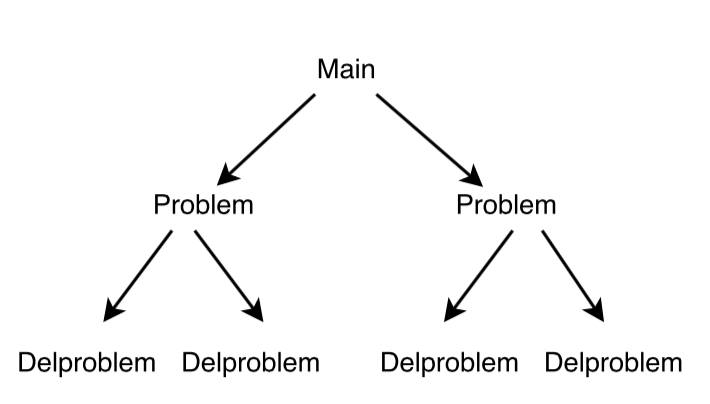
\includegraphics[width=10cm]{topdown}
    \caption{Tankegangen bag top-down programmering.}
    \label{fig:topdown}
\end{figure} 

\subsubsection{Programmets opbygning}

Programmet er opbygget efter desginprincippet "Top-down programmering". Princippet går ud på at dele programmet og i mindre dele, og derefter løse de mindre dele i hver deres funktion. Funktionerne samles i main, som kun bruges til kommunikation med brugeren. 

